\subsection{Nerd Sniping}
\index{Nerd Sniping}
\begin{figure}
\begin{center}
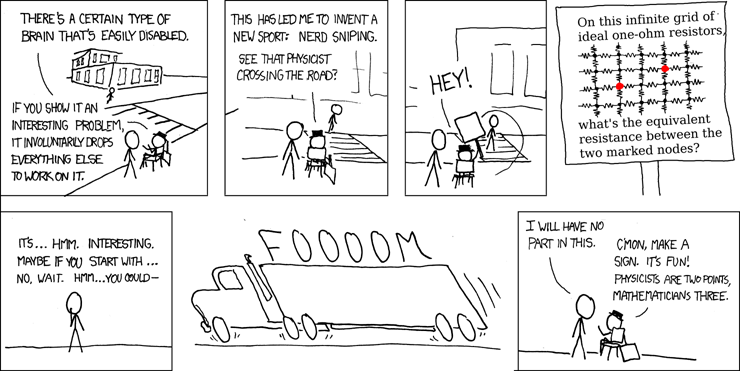
\includegraphics[width=\hsize]{graphics/nerdsniping}
\end{center}
\caption{Nerd Sniping nach Randall Munroe, {\tt xkcd.org}\label{nerdsniping}}
\end{figure}
Nerd Sniping ist ein von Randall Munroe erfundener Sport, wie
Abbildung~\ref{nerdsniping} zeigt. Im vorliegenden Fall soll
ein Nerd dadurch erledigt werden, dass man ihm die Aufgabe
stellt, den "Aquivalentwiderstand zwischen zwei beliebigen
Punkten eines unendlichen Widerstandsgitters zu berechnen.

\subsubsection{Problemstellung}
\begin{figure}
\begin{center}
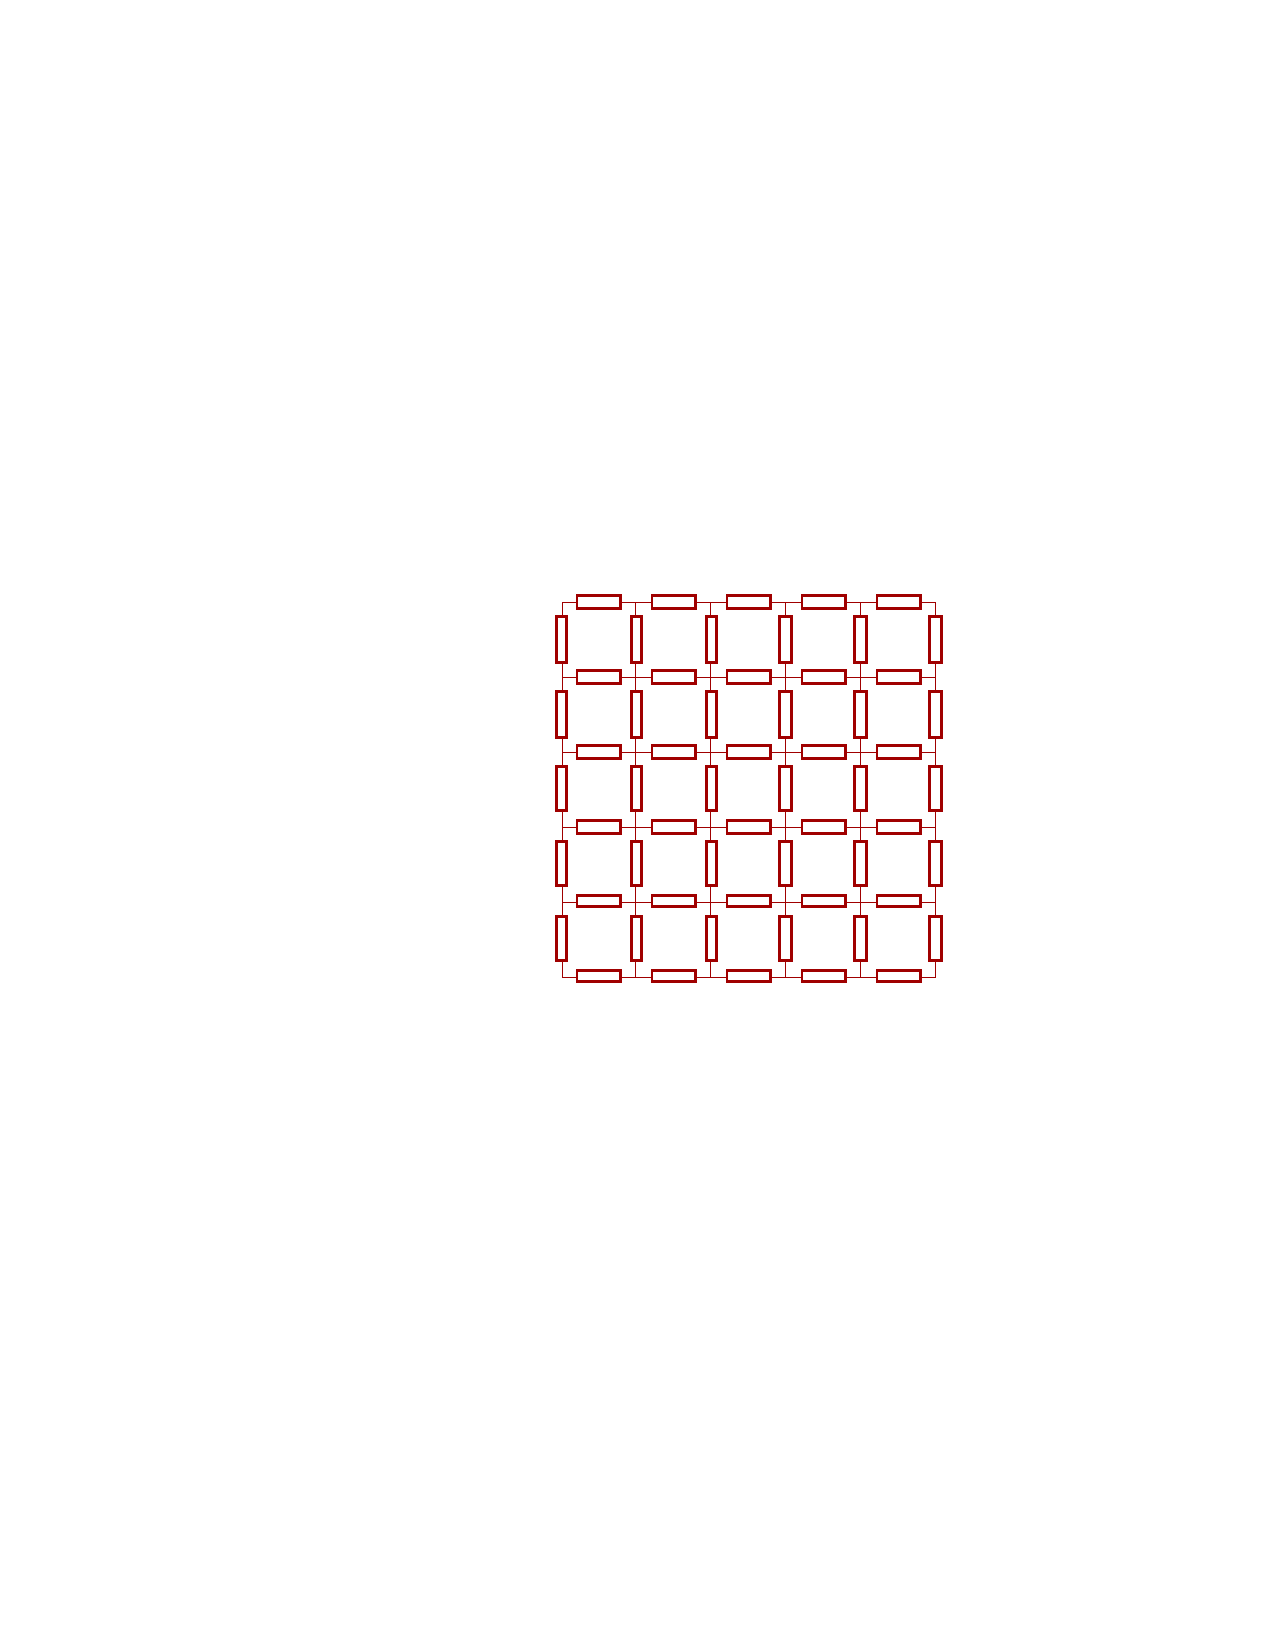
\includegraphics[width=0.6\hsize]{graphics/grid}
\end{center}
\caption{Widerstandsnetzwerk mit $n=5$\label{grid}}
\end{figure}
Gegeben ist ein quadratisches Gitter von $m\times m$ Punkten,
$m = n+1$, an denen ideale 1 Ohm Widerst"ande angeschlossen sind
(Abbildung~\ref{grid}).
In diesem Gitter sind offenbar $nm$ Widerst"ande in jeder Richtung
eingebaut, also insgesamt $2nm=2n(n+1)=2n^2+2n$ Widerst"ande.

Die Punkte des Gitters lassen sich mit
Zahlenpaaren $(i,j)$ adressieren, wobei wir uns gem"ass der bei Matrizen
"ublichen Konventionen die Zahl $i$ als Zeilenindex im Bereich $0\le i\le
n$ und die Zahl $j$ als Spaltenindex auch mit $0\le j\le n$ vorstellen.
Ausserdem sind zwei Gitterpunkte $P_1=(x_1,y_1)$ und $P_2=(x_2,y_2)$
gegeben. Gesucht ist der "Aquivalentwiderstand zwischen diesen beiden
Punkten.

\subsubsection{Reduktion auf ein lineares Gleichungssystem}
Um den Widerstand zu bestimmen, verbinden wir $P_1$ und $P_2$ mit den
Polen eine Stromquelle, die einen Strom von $1$A erzeugt. Der dabei
entstehende Potentialunterschied hat den gleichen Zahlenwert wie der
gesuchte "Aquivalentwiderstand. 

Zum Knoten $(i,j)$ geh"ort ein Potential $u_{ij}$, wir
k"onnen die Potentiale aber in Leserichtung zeilenweise von
links nach rechts und von oben nach unten anordnen, und in
einen Spaltenvektor $U$ packen.
Zu einem Gitter mit Kantenl"ange $n$ geh"ort dann
ein $m^2$-dimensionaler Vektor $U$.


Wir suchen also das Potential $U$ an den Knoten bei vorgegebenen
externen Str"omen aber ohne elektromotorische Kr"afte.
Im Abschnitt~\ref{appkirchhoff} hatten wir dazu Gleichung
(\ref{externestroeme}) gefunden. Der Laplace-Operator $\Delta$
ist besonders einfach auszurechnen, weil alle Widerst"ande den Wert
$1$ haben, $S$ ist die Einheitsmatrix.
F"ur ein $n\times n$-Gitter ist $\Delta$ eine $l\times l$-Matrix
mit $l=m^2$.

F"ur $n=4$ ist $m=5$ und $l=25$, wir erhalten eine $25\times 25$-Matrix
$\Delta_4$ wie in Abbildung~\ref{delta4}.
Es ist klar, dass der Vektor $U$ mit $U_i=1$ f"ur $0\le i<25$ im Nullraum
dieser Matrix ist, $\Delta_4 U=0$.
Wir wissen ja auch schon aus Abschnitt~\ref{appkirchhoff}, dass 
$\operatorname{Rang}\Delta_n=l-1$.

Da die Matrix aber auch symmetrisch ist, gilt auch $U^t\Delta_m=0$.
Die Gleichung $\Delta_nV=I_{\text{ext}}$ kann also nur dann eine
L"osung haben, wenn $U^tI_{\text{ext}}=0$ ist.
Physikalische bedeutet dies, dass alle
eingespeisten Str"ome sich zu 0 summieren, das Netzwerk sich 
also nicht aufladen kann.

%
% nerdmatrix.tex -- matrix für das Nerd Snipping Problem
%
% (c) 2017 Prof Dr Andreas Müller, Hochschule Rapperswil
%
\begin{landscape}
\begin{figure}
\[
\Delta_4=
\left(\begin{array}{ccccccccccccccccccccccccc}
   2& -1&   &   &   & -1&   &   &   &   &   &   &   &   &   &   &   &   &   &   &   &   &   &   &   \\
  -1&  3& -1&   &   &   & -1&   &   &   &   &   &   &   &   &   &   &   &   &   &   &   &   &   &   \\
    & -1&  3& -1&   &   &   & -1&   &   &   &   &   &   &   &   &   &   &   &   &   &   &   &   &   \\
    &   & -1&  3& -1&   &   &   & -1&   &   &   &   &   &   &   &   &   &   &   &   &   &   &   &   \\
    &   &   & -1&  2&   &   &   &   & -1&   &   &   &   &   &   &   &   &   &   &   &   &   &   &   \\
  -1&   &   &   &   &  3& -1&   &   &   & -1&   &   &   &   &   &   &   &   &   &   &   &   &   &   \\
    & -1&   &   &   & -1&  4& -1&   &   &   & -1&   &   &   &   &   &   &   &   &   &   &   &   &   \\
    &   & -1&   &   &   & -1&  4& -1&   &   &   & -1&   &   &   &   &   &   &   &   &   &   &   &   \\
    &   &   & -1&   &   &   & -1&  4& -1&   &   &   & -1&   &   &   &   &   &   &   &   &   &   &   \\
    &   &   &   & -1&   &   &   & -1&  3&   &   &   &   & -1&   &   &   &   &   &   &   &   &   &   \\
    &   &   &   &   & -1&   &   &   &   &  3& -1&   &   &   & -1&   &   &   &   &   &   &   &   &   \\
    &   &   &   &   &   & -1&   &   &   & -1&  4& -1&   &   &   & -1&   &   &   &   &   &   &   &   \\
    &   &   &   &   &   &   & -1&   &   &   & -1&  4& -1&   &   &   & -1&   &   &   &   &   &   &   \\
    &   &   &   &   &   &   &   & -1&   &   &   & -1&  4& -1&   &   &   & -1&   &   &   &   &   &   \\
    &   &   &   &   &   &   &   &   & -1&   &   &   & -1&  3&   &   &   &   & -1&   &   &   &   &   \\
    &   &   &   &   &   &   &   &   &   & -1&   &   &   &   &  3& -1&   &   &   & -1&   &   &   &   \\
    &   &   &   &   &   &   &   &   &   &   & -1&   &   &   & -1&  4& -1&   &   &   & -1&   &   &   \\
    &   &   &   &   &   &   &   &   &   &   &   & -1&   &   &   & -1&  4& -1&   &   &   & -1&   &   \\
    &   &   &   &   &   &   &   &   &   &   &   &   & -1&   &   &   & -1&  4& -1&   &   &   & -1&   \\
    &   &   &   &   &   &   &   &   &   &   &   &   &   & -1&   &   &   & -1&  3&   &   &   &   & -1\\
    &   &   &   &   &   &   &   &   &   &   &   &   &   &   & -1&   &   &   &   &  2& -1&   &   &   \\
    &   &   &   &   &   &   &   &   &   &   &   &   &   &   &   & -1&   &   &   & -1&  3& -1&   &   \\
    &   &   &   &   &   &   &   &   &   &   &   &   &   &   &   &   & -1&   &   &   & -1&  3& -1&   \\
    &   &   &   &   &   &   &   &   &   &   &   &   &   &   &   &   &   & -1&   &   &   & -1&  3& -1\\
    &   &   &   &   &   &   &   &   &   &   &   &   &   &   &   &   &   &   & -1&   &   &   & -1&  2
\end{array}\right)
\]
\caption{Laplace-Operator des Widerstandsgitters\label{delta4}}
\end{figure}
\end{landscape}


Die Tatsache, dass die Matrix symmetrisch ist, erlaubt zus"atzliche,
m"oglicherweise schnellere L"osungsverfahren anzuwenden, wie wir weiter
unten sehen werden.


\subsection{Numerische L"osung}
Eine numerische L"osung
muss zun"achst die Matrix $\Delta_n$ in geeigneter Form abspeichern.
%l"auft in folgenden Schritten ab:
%\begin{enumerate}
%\item Speicherplatz f"ur die Matrix $A_n$ allozieren und den Inhalt der Matrix setzen.
%\item Speicherplatz f"ur die rechte Seite $b$ allozieren und den Inhalt setzen.
%\item L"osungsalgorithmus aus der Bibliothek aufrufen.
%\item Spannung zwischen den Punkten $P_i$ berechnen.
%\end{enumerate}
Um die gesamte Matrix $\Delta_m$ zu speichern, braucht man $l^2=m^4$
Speicherpl"atze%
\footnote{Da die Bibliotheken typischerweise
L"osungsfunktionen f"ur single precision oder double precision
enthalten, wollen wir uns bez"uglich der Gr"osse eines Speicherplatzes
nicht festlegen. Rechnet man mit double precision, wird man in C
den Datentyp {\tt double} verwenden, der normalerweise 8 Bytes Platz
beansprucht. $10^9$ Speicherpl"atze entsprechen in diesem Falle also
etwa 8 GB.}.  Aus Tabelle \ref{bedarf} kann man ablesen, dass sich mit
dieser Methode nur Probleme mit $n\le 174$ bearbeiten lassen.

In der Matrix sind in den $n^2$ Gleichungen f"ur die inneren Punkte
$5$ Elemente von $0$ verschieden, f"ur die $4n$ Gleichungen f"ur
Randpunkte jedoch nur $4$ Elemente, und f"ur die $4$ Ecken sogar nur $3$
Elemente. Grunds"atzlich w"are es also m"oglich, die gesamte Information
in $ 5n^2+16n+12$ Speicherpl"atzen unterzubringen.  Die Matrizen $A_n$
sind also extrem d"unn besetzt (englisch ``sparse'').

Das Beispiel f"ur $n=4$ zeigt auch, dass die Matrix Bandstruktur hat. Mehr
als $n$ Elemente von der Diagonalen entfernt sind alle Matrixelemente
$0$. Es w"urde also auch reichen, nur die Elemente innerhalb eines Bandes
der Breite $\pm n$ um die Diagonale zu speichern.  Dazu sind $(2n+1)l -
2m^2+m=(2m-1)m^2-2m^2+m=2m^3-3m^2+m$ Speicherpl"atze n"otig.

In allen F"allen l"asst sich der ben"otige Speicherplatz nochmals um
den Faktor 2 reduzieren, falls man die Symmetrie der Matrix ausnutzen
kann. Dies ist jedoch nicht immer m"oglich. Die Matrix $A_n$ ist
singul"ar, genauer, sie hat Rang $l-1$.  Daher kann es f"ur einen
gegebenen Algorithmus n"otig sein, eine der Gleichungen durch eine neue
zu ersetzen, die zum Beispiel den Wert der letzten Variablen $u_{nn}$
festlegt,
\[
u_{nn}=0,
\]
Dadurch wird aber die Symmetrie der Matrix zerst"ort.

\begin{table}
\begin{center}
\begin{tabular}{|lr|c|r|}
\hline
Methode&&Platzbedarf&$n$ f"ur $10^9$ Speicherpl"atze\\
\hline
Voll&{\tt dgesv}&$m^4$&176\\
Bandstruktur&{\tt dgbsv}&$2m^3$&793\\
d"unn besetzt&{\tt CGIter}&$5m^2$&14140\\
\hline
\end{tabular}
\end{center}
\caption{Speicherplatzbedarf und maximale Problemgr"osse $n$, die mit $10^9$
Speicherpl"atzen bearbeitet werden kann.\label{bedarf}}
\end{table}

\subsubsection{Mit LAPACK}
LAPACK ist eine frei verf"ugbare Bibliothek zur numerischen L"osung 
vieler Probleme der linearen Algebra. 
Man findet die Software auf dem Internet\footnote{\small\tt http://www.netlib.org/lapack/}, die Dokumentation in HTML-Format
kann unter
{\small\tt http://www.netlib.org/lapack/lug/} abgerufen werden.

Urspr"unglich ist LAPACK in Fortran geschrieben.
Festgelegt ist nur das API,
so dass auch Implementationen in anderen Sprachen m"oglich sind.
Auch stellen verschiedene
Hersteller optimierte Versionen von LAPACK bereit.
Auf Unix-Systemen geh"ort LAPACK zum Standardumfang
des Betriebssystems, sogar jedes iPhone und iPad beinhalten LAPACK.
Intel bietet eine Version an, die die F"ahigkeiten der Intel-Prozessoren
optimal ausn"utzen, und zum Beispiel mit so vielen parallelen Threads
wie m"oglich arbeitet.

Die Routinen von LAPACK k"onnen volle Matrizen oder Bandmatrizen
bearbeiten, es gibt aber in LAPACK keine M"oglichkeit, d"unn besetzte
Matrizen platzsparend zu speichern. Daher wird man mit LAPACK nur Probleme
mit $n$ bis h"ochstens etwa 700 l"osen k"onnen, wobei man f"ur $n\ge 200$
die Bandstruktur verwenden muss.

\medskip
{\parindent0pt
{\bf Volle Matrix.}}
Die Funktion {\tt dgesv\_} berechnet die L"osung eines Gleichungssystems mit 
einer voll besetzten Matrix. Diese Funktion kann die Gleichungen auch
bei Rang $l-1$ l"osen, so dass es nicht unbedingt n"otig ist, die letzte
Gleichung durch $u_{nn}=0$ zu ersetzen.

Zur Speicherung der vollen Matrix verwenden wir einen {\tt double}-Array mit $l^2$ Elementen.
Die Gleichung zu einem inneren Punkt $(i,j)$ wird dann mit folgendem Code 
in die Matrix eingef"ugt.
\verbatiminput{applications/lapackaf.c}
"Ahnlicher Code wird f"ur den Rest der Matrix verwendet.

\medskip
{\parindent0pt
{\bf Bandmatrix.}}
Die Funktion {\tt dgbsv\_} kann Gleichungssysteme mit Bandmatrizen
l"osen. Auch in diesem Fall ist es nicht n"otig, $u_{nn}=0$ hinzuzuf"ugen.

F"ur die Speicherung der Matrix braucht man ebenfalls einen {\tt
double}-Array, der aber anders adressiert wird. Die Details zur Besetzung
dieses Arrays werden in der LAPACK-Dokumentation dargestellt. F"ur das
Programm k"onnen wir diese zus"atzliche Komplexit"at wieder in zwei
Macros verbergen, so wie wir schon im Falle der vollen Matrix Macros
zur Adressierung des Arrays verwendet haben.
\verbatiminput{applications/lapackab.c}
Die Zahlen {\tt kl} und {\tt ku} bezeichnen die Breite des Bandes oberhalb
({\tt ku}) und unterhalb ({\tt kl}) der Diagonalen. {\tt ldab} ist die
vertikale Dimension der Matrix, in der man die Bandmatrix "ubergeben
muss. Sie ist etwas gr"osser als minimal n"otig, da LAPACK noch etwas
Platz f"ur die Durchf"uhrung der Rechnung ben"otigt.

\subsubsection{Mit LASPACK}
LASPACK ist eine Bibliothek von Tom\'a\v s Skalick\'y, welche L"osungen
d"unn besetzter linearer Gleichungssysteme berechnen kann. Solch grosse
Gleichungssysteme k"onnen effizient mit iterativen Methoden gel"ost
werden.

Die Speicherung von d"unn besetzten Matrizen erfolgt zeilenweise. Zu
jeder Zeile muss festgelegt werden, wie viele Elemente von 0 verschieden
sind, und es m"ussen deren Werte zusammen mit der Position innerhalb
der Zeile gespeichert werden.  Um also eine Zeile zu speichern, die zu
einem inneren Punkt geh"ort, ist der folgende Code notwendig:
\verbatiminput{applications/laspacka.c}
Dabei wird ber"ucksichtigt, dass wir mit Indizes zwischen $0$ und $l-1$
arbeiten, w"ahrend LASPACK mit Indizes zwischen $1$ und $l$ arbeitet. Der
Macro {\tt A} speichert den neuen Wert im jeweils n"achsten freien Platz
auf der Zeile.

Da die Matrix $A_n$ symmetrisch ist, kann die Methode der konjugierten
Gradienten verwendet werden.  Die Implementation von LASPACK erlaubt
auch, den Nullraum der Matrix anzugeben (aufgespannt durch den Vektor $U$),
die Methode {\tt CGIter} findet dann eine L"osung
des Gleichungssystems, die orthogonal auf $v$ ist.

\subsubsection{Resultate}
Zum Vergleich der verschiedenen Implementationen wurde Laufzeit
und der Widerstand zwischen zwei gegen"uberliegenden Ecken des
Widerstandsgitters in Abh"angigkeit von $n$ f"ur $n$ zwischen $10$ und
$1100$ ermittelt. Speicherplatzbedarf aber auch Laufzeit haben dabei
verhindert, dass die langsamen Algorithmen bis $n=1100$ gemessen werden
konnten. Die gemessenen maximalen $n$ sind in Tabelle~\ref{results}
zusammengefasst.

\medskip
{\parindent0pt
{\bf Widerstand.}}
\begin{figure}
\begin{center}
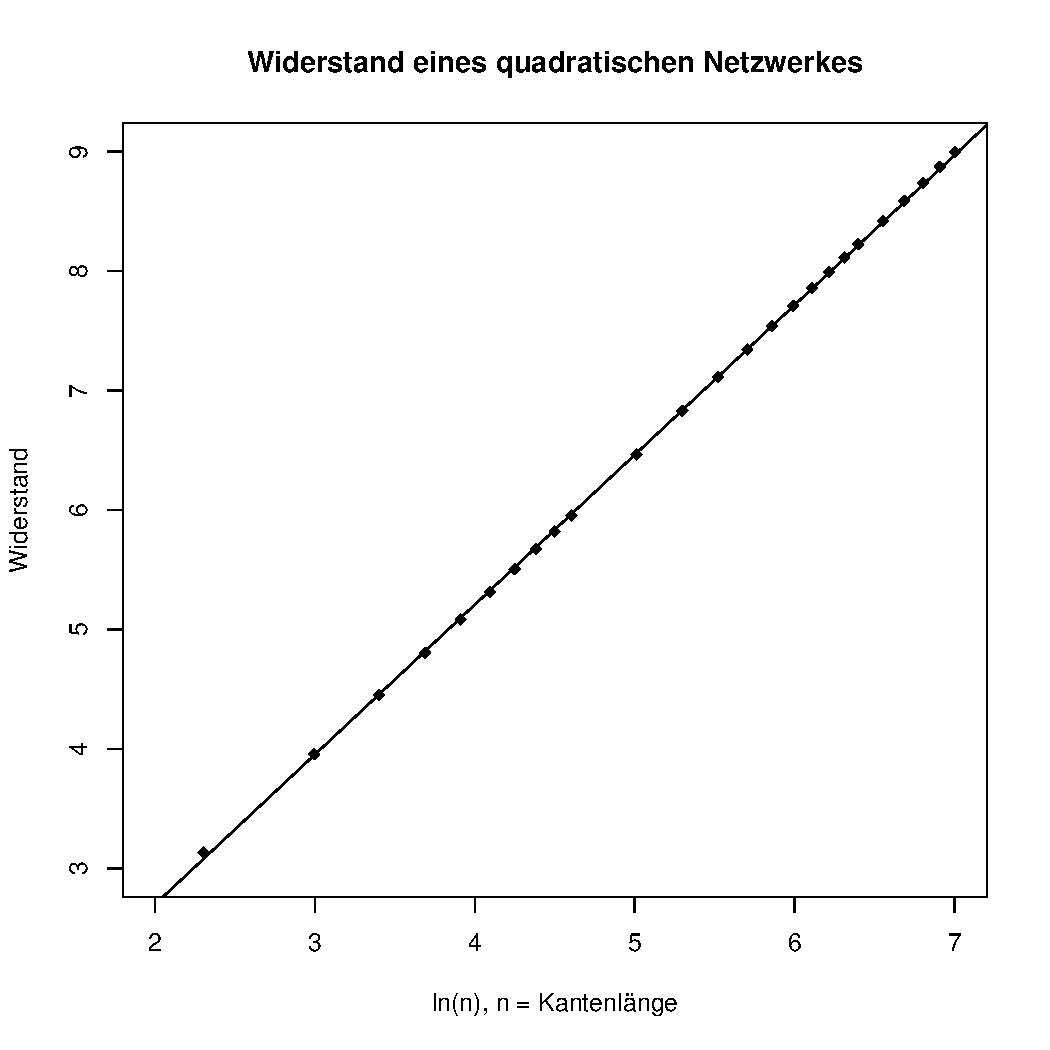
\includegraphics[width=\hsize]{graphics/resistance}
\end{center}
\caption{Gesamtwiderstand (zwischen gegen"uberliegenden Ecken)
in Abh"angigkeit von der Kantenl"ange $n$,
logarithmische Skala\label{resistance}}
\end{figure}
F"ur den Widerstand zwischen zwei gegen"uberliegenden Ecken des
in Abh"angigkeit von der Kantenl"ange findet man die in
Abbildung~\ref{resistance} dargestellten Resultate. Lineare Regression 
ergibt eine Steigung von $1.2543$, was die Vermutung nahelegt, dass der
Widerstand $R$ des Netzwerkes asymptotisch wie $e^{\frac54n}$ w"achst.

\begin{figure}
\begin{center}
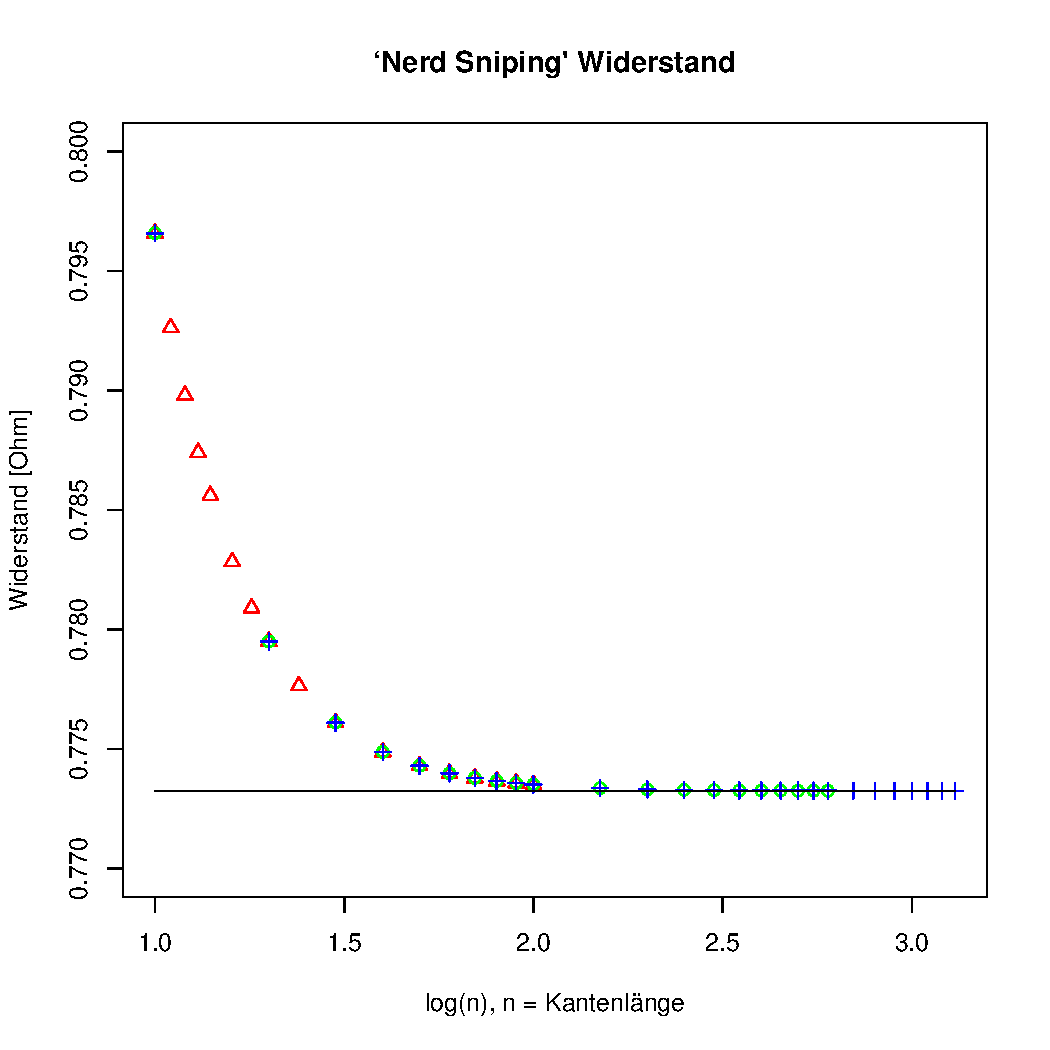
\includegraphics[width=\hsize]{graphics/snipingresistance}
\end{center}
\caption{Widerstand in Abh"angigkeit von $n$\label{snipingresistance}}
\end{figure}
Mit Hilfe des Programms kann jetzt auch die urspr"ungliche Frage von
Randall Munroe beantwortet werden. Abbildung~\ref{snipingresistance} zeigt
den Widerstand zwischen den Punkten $P_{ns,1}=(\frac{n}2-1,\frac{n}2)$ und
$P_{ns,2}=(\frac{n}2+1,\frac{n}2+1)$. Offenbar konvergiert der Widerstand
gegen einen Wert von ungef"ahr $R\simeq 0.773241$.  Die Konvergenz
ist nicht unerwartet.  Die weit von $P_{ns,i}$ entfernten Widerst"ande
k"onnen nur von einem sehr geringen Strom durchflossen werden, denn die
Potentialdifferenz zwischen den Punkten $P_{ns,i}$ f"allt "uber eine
grosse Zahl von Widerst"anden auf dem Weg von $P_{ns,1}$ "uber den zum
besagten Widerstand und zur"uck zu $P_{ns,2}$ ab, so dass die einzelnen
Spannungsabf"alle notwendigerweise umso geringer sind, je weiter entfernt
ein Widerstand ist.


{\bf Laufzeit.}
\begin{figure}
\begin{center}
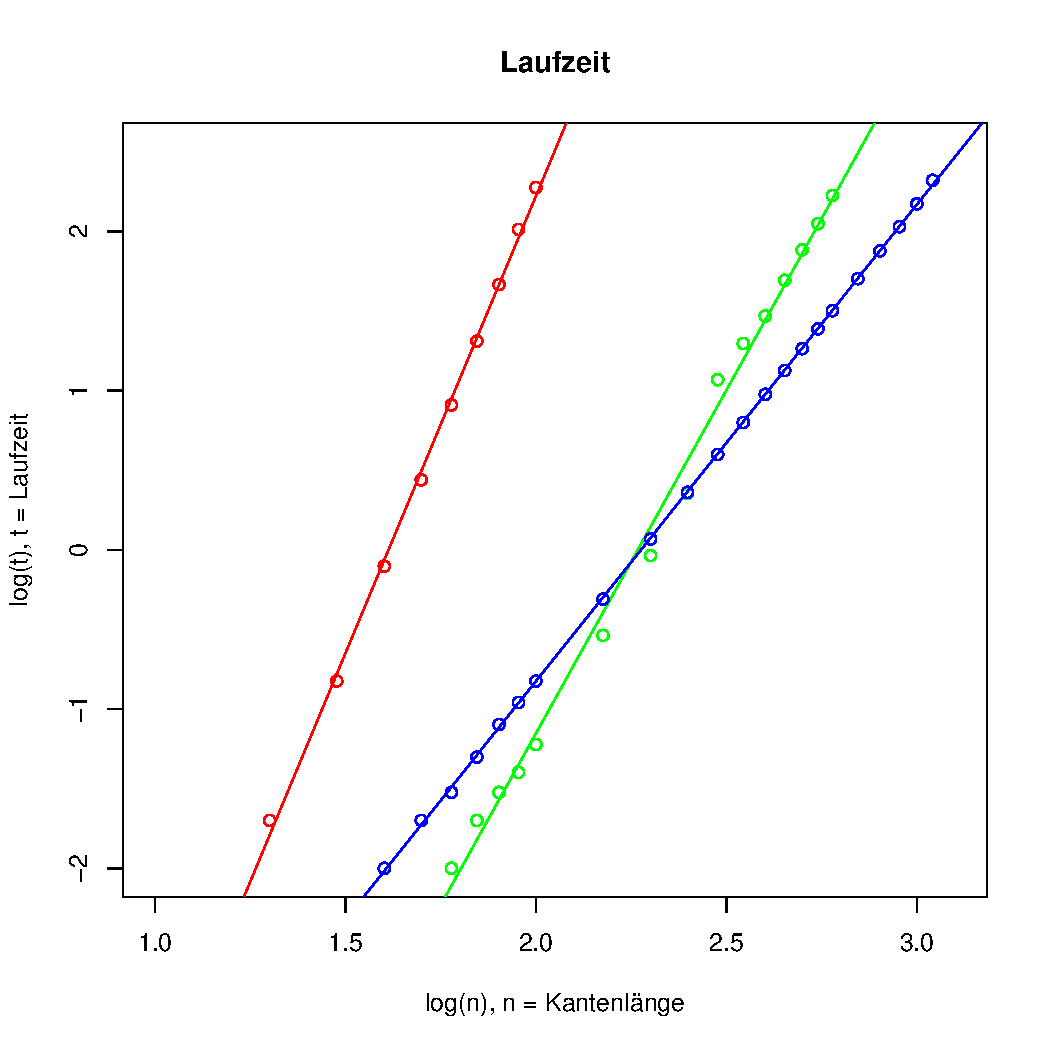
\includegraphics[width=\hsize]{graphics/runtime}
\end{center}
\caption{Laufzeit verschiedener Algorithmen: LAPACK {\tt dgesv} (rot),
LAPACK {\tt dgbsv} (gr"un)
und LASPACK {\tt CGIter} (blau)\label{runtime}}
\end{figure}
Performance-Messungen wurden auf einem MacBook Pro mit 8GB RAM und
einem 2 GHz Intel Core i7 Prozessor durchgef"uhrt. Dabei fiel auf, dass
die LAPACK-Library von Mac OS X die vorhanden Cores nach M"oglichkeit
ausn"utzt. Im {\tt dgesv}-Algorithmus wurden 8 Threads genutzt, die
CPU also voll ausgelastet, bei {\tt dgbsv} dagegen nur 3-4 Threads.
Die LASPACK-Bibliothek ist nicht multithreaded, hier wird immer nur ein
Thread genutzt. Die absoluten Laufzeiten der Algorithmen sind daher nur
bedingt vergleichbar.


Die Laufzeiten der verschiedenen Algorithmen h"angen im wesentlichen
polynomiell von der Problemgr"osse ab, wie man in Abbildung \ref{runtime}
erkennen kann.  Es ist bekannt, dass der Gauss-Algorithmus Komplexit"at
$O(n^3)$ hat, da in unserem Fall aber die Problemgr"osse $l=O(n^2)$ ist,
erwartet man den Exponenten $O(n^6)$ f"ur die Komplexit"at der L"osung
mit der Methode {\tt dgesv}.

Die Ausn"utzung der Bandmatrizen-Struktur reduziert die Komplexit"at des
Gauss-Algorithmus auf $O(ln^2)=O(n^4)$. Die Komplexit"at des konjugierte
Gradienten Algorithmus scheint $O(n^3)$ zu sein.
\begin{table}
\begin{center}
\begin{tabular}{|l|crrr|}
\hline
Methode&Threads&Exponent&vermutet&$n_{\text{max}}$\\
\hline
{\tt dgesv}&8&5.742&6&100\\
{\tt dgbsv}&3&4.331&4&600\\
{\tt CGIter}&1& 2.993&3&1100\\
\hline
\end{tabular}
\end{center}
\caption{Laufzeiten und Exponenten der Abh"angigkeit von $n$\label{results}}
\end{table}
